\documentclass[dvipdfmx]{jarticle}
\pagestyle{empty}
\usepackage{tikz}
\usetikzlibrary{shapes,calc}
\begin{document}
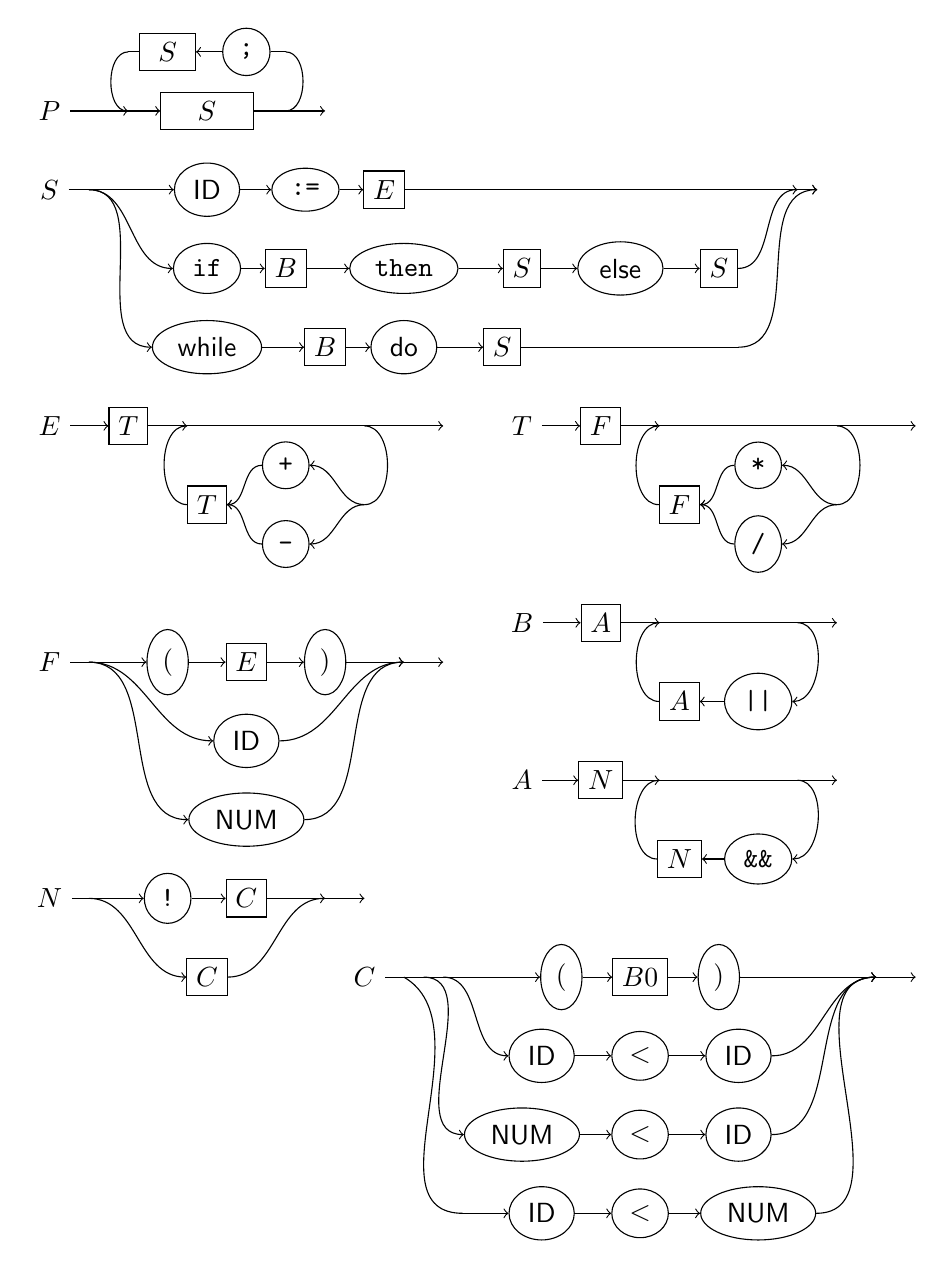
\begin{tikzpicture}
  \node (P0) at (0,0) {$P$};
  \node[draw] (P1) at ($(P0)+(2,0)$) {\mbox{\quad $S$\quad }};
  \node[draw,circle] (P2) at ($(P1)+(0.5,0.75)$) {\texttt{;}};
  \node[draw,rectangle] (P3) at ($(P1)+(-0.5,0.75)$) {\mbox{\ $S$\ }};
  \path[->] (P0) edge (P1);
  \path[->] (P1) edge ($(P1)+(1.5,0)$);
  \path[-] ($(P1)+(1,0)$) [out=0,in=0] edge ($(P1)+(1,0.75)$);
  \path[-] ($(P1)+(1,0.75)$) edge (P2);
  \path[->] (P2) edge (P3);
  \path[-] (P3) edge ($(P3)+(-0.5,0)$);
  \path[->] ($(P3)+(-0.5,0)$) [out=180,in=180] edge ($(P1)+(-1,0)$);
  %\node (S0) at (0,-1) {$S$};
  
  \coordinate (S0) at ($(P0)+(1,-1)$);
  \node (S-1) at ($(S0)+(-1,0)$) {$S$};
  \node[draw,ellipse] (S1) at ($(S0)+(1,0)$) {{\sf ID}};
  \node[draw,ellipse] (S11) at ($(S1)+(1.25,0)$) {\texttt{:=}};
  \node[draw] (S12) at ($(S11)+(1,0)$) {$E$};
  \node[draw,ellipse] (S2) at ($(S1)+(0,-1)$) {\texttt{if}};
  \node[draw] (S21) at ($(S2)+(1,0)$) {$B$};
  \node[draw,ellipse] (S22) at ($(S21)+(1.5,0)$) {\texttt{then}};
  \node[draw] (S23) at ($(S22)+(1.5,0)$) {$S$};
  \node[draw,ellipse] (S24) at ($(S23)+(1.25,0)$) {{\sf else}};
  \node[draw] (S25) at ($(S24)+(1.25,0)$) {$S$};
  \node[draw,ellipse] (S3) at ($(S0)+(1,-2)$) {{\sf while}};
  \node[draw] (S31) at ($(S3)+(1.5,0)$) {$B$};
  \node[draw,ellipse] (S32) at ($(S31)+(1,0)$) {{\sf do}};
  \node[draw] (S33) at ($(S32)+(1.25,0)$) {$S$};
  \path[->] (S-1) edge (S1) (S1) edge (S11) (S11) edge (S12) (S12) edge ($(S12)+(5.5,0)$);
  \path[->,out=0,in=180] ($(S0)+(-0.5,0)$) edge (S2);
  \path[->] (S2) edge (S21) (S21) edge (S22) (S22) edge (S23) (S23) edge (S24)
    (S24) edge (S25);
  \path[->,out=0,in=180] (S25) edge ($(S25)+(1,1)$);
  \path[->,out=0,in=180] ($(S0)+(-0.5,0)$) edge (S3);
  \path[->] (S3) edge (S31) (S31) edge (S32) (S32) edge (S33);
  \path[-] (S33) edge ($(S33)+(3,0)$);
  \path[->,out=0,in=180] ($(S33)+(3,0)$) edge ($(S33)+(4,2)$);

  \node (E0) at ($(P0)+(0,-4)$) {$E$};
  \node[draw] (E1) at ($(E0)+(1,0)$) {$T$};
  \node[draw,ellipse] (E11) at ($(E1)+(2,-0.5)$) {\texttt{+}};
  \node[draw,ellipse] (E12) at ($(E11)+(0,-1)$) {\texttt{-}};
  \node[draw] (E13) at ($(E11)+(-1,-0.5)$) {$T$};
  \path[->] (E0) edge (E1) (E1) edge ($(E1)+(4,0)$);
  \path[-,out=0,in=0] ($(E1)+(3,0)$) edge ($(E1)+(3,-1)$);
  \path[->,out=180,in=0] ($(E1)+(3,-1)$) edge (E11)
    ($(E1)+(3,-1)$) edge (E12);
  \path[->,out=180,in=0] (E11) edge (E13);
  \path[->,out=180,in=0] (E12) edge (E13);
  \path[->,out=180,in=180] (E13) edge ($(E1)+(0.75,0)$);

  \node (T0) at ($(P0)+(6,-4)$) {$T$};
  \node[draw] (T1) at ($(T0)+(1,0)$) {$F$};
  \node[draw,ellipse] (T11) at ($(T1)+(2,-0.5)$) {\texttt{*}};
  \node[draw,ellipse] (T12) at ($(T11)+(0,-1)$) {\texttt{/}};
  \node[draw] (T13) at ($(T11)+(-1,-0.5)$) {$F$};
  \path[->] (T0) edge (T1) (T1) edge ($(T1)+(4,0)$);
  \path[-,out=0,in=0] ($(T1)+(3,0)$) edge ($(T1)+(3,-1)$);
  \path[->,out=180,in=0] ($(T1)+(3,-1)$) edge (T11)
    ($(T1)+(3,-1)$) edge (T12);
  \path[->,out=180,in=0] (T11) edge (T13);
  \path[->,out=180,in=0] (T12) edge (T13);
  \path[->,out=180,in=180] (T13) edge ($(T1)+(0.75,0)$);

  \node (F0) at ($(P0)+(0,-7)$) {$F$};
  \node[draw,ellipse] (F1) at ($(F0)+(1.5,0)$) {$($};
  \node[draw] (F11) at ($(F1)+(1,0)$) {$E$};
  \node[draw,ellipse] (F12) at ($(F11)+(1,0)$) {$)$};
  \node[draw,ellipse] (F2) at ($(F11)+(0,-1)$) {$\mathsf{ID}$};
  \node[draw,ellipse] (F3) at ($(F2)+(0,-1)$) {$\mathsf{NUM}$};
  \path[->] (F0) edge (F1) (F1) edge (F11) (F11) edge (F12) (F12) edge ($(F12)+(1.5,0)$);
  \path[->,out=0,in=180] ($(F0)+(0.5,0)$) edge (F2);
  \path[->,out=0,in=180] (F2) edge ($(F12)+(1,0)$);
  \path[->,out=0,in=180] ($(F0)+(0.5,0)$) edge (F3);
  \path[->,out=0,in=180] (F3) edge ($(F12)+(1,0)$);

  \node (B0) at ($(P0)+(6,-6.5)$) {$B$};
  \node[draw] (B1) at ($(B0)+(1,0)$) {$A$};
  \node[draw,ellipse] (B11) at ($(B1)+(2,-1)$) {$\texttt{||}$};
  \node[draw] (B12) at ($(B11)+(-1,0)$) {$A$};
  \path[->] (B0) edge (B1) (B1) edge ($(B1)+(3,0)$);
  \path[->,out=0,in=0] ($(B1)+(2.5,0)$) edge (B11);
  \path[->] (B11) edge (B12);
  \path[->,out=180,in=180] (B12) edge ($(B1)+(0.75,0)$);

  \node (A0) at ($(P0)+(6,-8.5)$) {$A$};
  \node[draw] (A1) at ($(A0)+(1,0)$) {$N$};
  \node[draw,ellipse] (A11) at ($(A1)+(2,-1)$) {$\texttt{\&\&}$};
  \node[draw] (A12) at ($(A11)+(-1,0)$) {$N$};
  \path[->] (A0) edge (A1) (A1) edge ($(A1)+(3,0)$);
  \path[->,out=0,in=0] ($(A1)+(2.5,0)$) edge (A11);
  \path[->] (A11) edge (A12);
  \path[->,out=180,in=180] (A12) edge ($(A1)+(0.75,0)$);

  \node (N0) at ($(P0)+(0,-10)$) {$N$};
  \node[draw,ellipse] (N1) at ($(N0)+(1.5,0)$) {\texttt{!}};
  \node[draw] (N11) at ($(N1)+(1,0)$) {$C$};
  \node[draw] (N2) at ($(N11)+(-0.5,-1)$) {$C$};
  \path[->] (N0) edge (N1) (N1) edge (N11) (N11) edge ($(N11)+(1.5,0)$);
  \path[->,out=0,in=180] ($(N0)+(0.5,0)$) edge (N2);
  \path[->,out=0,in=180] (N2) edge ($(N11)+(1,0)$);

  \node (C0) at ($(P0)+(4,-11)$) {$C$};
  \node[draw,ellipse] (C1) at ($(C0)+(2.5,0)$) {$($};
  \node[draw] (C11) at ($(C1)+(1,0)$) {$B$0};
  \node[draw,ellipse] (C12) at ($(C11)+(1,0)$) {$)$};
  \node[draw,ellipse] (C2) at ($(C1)+(-0.25,-1)$) {$\mathsf{ID}$};
  \node[draw,ellipse] (C21) at ($(C11)+(0,-1)$) {$\mathsf{<}$};
  \node[draw,ellipse] (C22) at ($(C12)+(0.25,-1)$) {$\mathsf{ID}$};
  \node[draw,ellipse] (C3) at ($(C2)+(-0.25,-1)$) {$\mathsf{NUM}$};
  \node[draw,ellipse] (C31) at ($(C21)+(0,-1)$) {$\mathsf{<}$};
  \node[draw,ellipse] (C32) at ($(C22)+(0,-1)$) {$\mathsf{ID}$};
  \node[draw,ellipse] (C4) at ($(C3)+(0.25,-1)$) {$\mathsf{ID}$};
  \node[draw,ellipse] (C41) at ($(C31)+(0,-1)$) {$\mathsf{<}$};
  \node[draw,ellipse] (C42) at ($(C32)+(0.25,-1)$) {$\mathsf{NUM}$};
  \path[->] (C0) edge (C1) (C1) edge (C11) (C11) edge (C12) (C12) edge ($(C12)+(2.5,0)$);
  \path[->,out=0,in=180] ($(C0)+(1,0)$) edge (C2);
  \path[->] (C2) edge (C21) (C21) edge (C22);
  \path[->,out=0,in=180] (C22) edge ($(C12)+(2,0)$);
  \path[->,out=0,in=180] ($(C0)+(0.75,0)$) edge (C3);
  \path[->] (C3) edge (C31) (C31) edge (C32);
  \path[->,out=0,in=180] (C32) edge ($(C12)+(2,0)$);
  \path[-,out=-30,in=180] ($(C0)+(0.5,0)$) edge ($(C4)+(-1,0)$);
  \path[->] ($(C4)+(-1,0)$) edge (C4);
  \path[->] (C4) edge (C41) (C41) edge (C42);
  \path[->,out=0,in=180] (C42) edge ($(C12)+(2,0)$);
\end{tikzpicture}
\end{document}